% Checked scored-data replay; not publication approval.
% canonical observations SHA-256: 1b1c1957cc120d30c257ebc4523437ba3395ab470d98556b0b79b376b25790c6
\newcommand{\PfAccCOne}{12.4}
\newcommand{\PfAccLoCOne}{9.8}
\newcommand{\PfAccHiCOne}{15.6}
\newcommand{\PfNCOne}{500}
\newcommand{\PfCorrectCOne}{62}
\newcommand{\PfTokCOne}{1,022}
\newcommand{\PfSecsCOne}{17.4}
\newcommand{\PfCapHitsCOne}{0}
\newcommand{\PfUnclosedCOne}{0}
\newcommand{\PfMissingCOne}{0}
\newcommand{\PfJudgeAgreeCOne}{98.2}
\newcommand{\PfJudgeKappaCOne}{0.91}
\newcommand{\PfContAccCOne}{12.3}
\newcommand{\PfContAgreeCOne}{90.5}
\newcommand{\PfDiagChunksCOne}{245.8}
\newcommand{\PfDiagEvidenceWordRecallCOne}{4.8}
\newcommand{\PfDiagFallbackChunksDroppedCOne}{56.4}
\newcommand{\PfDiagHistoryCharsKeptCOne}{3,877.8}
\newcommand{\PfDiagPercentileCOne}{99.0}
\newcommand{\PfDiagSelectionSecondsCOne}{0.04}
\newcommand{\PfDiagCountFallbackCOne}{500}
\newcommand{\PfAccCFour}{25.2}
\newcommand{\PfAccLoCFour}{21.6}
\newcommand{\PfAccHiCFour}{29.2}
\newcommand{\PfNCFour}{500}
\newcommand{\PfCorrectCFour}{126}
\newcommand{\PfTokCFour}{3,559}
\newcommand{\PfSecsCFour}{24.9}
\newcommand{\PfCapHitsCFour}{1}
\newcommand{\PfUnclosedCFour}{0}
\newcommand{\PfMissingCFour}{0}
\newcommand{\PfJudgeAgreeCFour}{98.0}
\newcommand{\PfJudgeKappaCFour}{0.95}
\newcommand{\PfContAccCFour}{22.0}
\newcommand{\PfContAgreeCFour}{86.8}
\newcommand{\PfDiagChunksCFour}{245.8}
\newcommand{\PfDiagEvidenceWordRecallCFour}{26.3}
\newcommand{\PfDiagFallbackChunksDroppedCFour}{0.0}
\newcommand{\PfDiagHistoryCharsKeptCFour}{16,714.3}
\newcommand{\PfDiagPercentileCFour}{97.0}
\newcommand{\PfDiagSelectionSecondsCFour}{0.42}
\newcommand{\PfDiagCountFallbackCFour}{0}
\newcommand{\PfAccCwOne}{10.6}
\newcommand{\PfAccLoCwOne}{8.2}
\newcommand{\PfAccHiCwOne}{13.6}
\newcommand{\PfNCwOne}{500}
\newcommand{\PfCorrectCwOne}{53}
\newcommand{\PfTokCwOne}{1,005}
\newcommand{\PfSecsCwOne}{10.1}
\newcommand{\PfCapHitsCwOne}{0}
\newcommand{\PfUnclosedCwOne}{0}
\newcommand{\PfMissingCwOne}{0}
\newcommand{\PfJudgeAgreeCwOne}{98.2}
\newcommand{\PfJudgeKappaCwOne}{0.90}
\newcommand{\PfContAccCwOne}{10.9}
\newcommand{\PfContAgreeCwOne}{90.2}
\newcommand{\PfDiagChunksCwOne}{10.4}
\newcommand{\PfDiagEvidenceWordRecallCwOne}{12.3}
\newcommand{\PfDiagFallbackChunksDroppedCwOne}{0.0}
\newcommand{\PfDiagHistoryCharsKeptCwOne}{5,442.0}
\newcommand{\PfDiagPercentileCwOne}{77.8}
\newcommand{\PfDiagSelectionSecondsCwOne}{0.02}
\newcommand{\PfDiagWindowTokensCwOne}{4,317.0}
\newcommand{\PfDiagCountFallbackCwOne}{0}
\newcommand{\PfAccCwFour}{20.0}
\newcommand{\PfAccLoCwFour}{16.7}
\newcommand{\PfAccHiCwFour}{23.7}
\newcommand{\PfNCwFour}{500}
\newcommand{\PfCorrectCwFour}{100}
\newcommand{\PfTokCwFour}{4,017}
\newcommand{\PfSecsCwFour}{18.0}
\newcommand{\PfCapHitsCwFour}{0}
\newcommand{\PfUnclosedCwFour}{1}
\newcommand{\PfMissingCwFour}{0}
\newcommand{\PfJudgeAgreeCwFour}{96.4}
\newcommand{\PfJudgeKappaCwFour}{0.88}
\newcommand{\PfContAccCwFour}{18.4}
\newcommand{\PfContAgreeCwFour}{85.9}
\newcommand{\PfDiagChunksCwFour}{38.7}
\newcommand{\PfDiagEvidenceWordRecallCwFour}{37.3}
\newcommand{\PfDiagFallbackChunksDroppedCwFour}{0.0}
\newcommand{\PfDiagHistoryCharsKeptCwFour}{23,116.3}
\newcommand{\PfDiagPercentileCwFour}{75.3}
\newcommand{\PfDiagSelectionSecondsCwFour}{0.09}
\newcommand{\PfDiagWindowTokensCwFour}{16,596.4}
\newcommand{\PfDiagCountFallbackCwFour}{0}
\newcommand{\PfAccENo}{8.6}
\newcommand{\PfAccLoENo}{6.4}
\newcommand{\PfAccHiENo}{11.4}
\newcommand{\PfNENo}{500}
\newcommand{\PfCorrectENo}{43}
\newcommand{\PfTokENo}{57}
\newcommand{\PfSecsENo}{6.7}
\newcommand{\PfCapHitsENo}{0}
\newcommand{\PfUnclosedENo}{0}
\newcommand{\PfMissingENo}{0}
\newcommand{\PfJudgeAgreeENo}{99.4}
\newcommand{\PfJudgeKappaENo}{0.96}
\newcommand{\PfContAccENo}{7.7}
\newcommand{\PfContAgreeENo}{93.0}
\newcommand{\PfAccMOne}{39.0}
\newcommand{\PfAccLoMOne}{34.8}
\newcommand{\PfAccHiMOne}{43.3}
\newcommand{\PfNMOne}{500}
\newcommand{\PfCorrectMOne}{195}
\newcommand{\PfTokMOne}{756}
\newcommand{\PfSecsMOne}{9.7}
\newcommand{\PfCapHitsMOne}{0}
\newcommand{\PfUnclosedMOne}{0}
\newcommand{\PfMissingMOne}{0}
\newcommand{\PfJudgeAgreeMOne}{96.8}
\newcommand{\PfJudgeKappaMOne}{0.93}
\newcommand{\PfContAccMOne}{34.8}
\newcommand{\PfContAgreeMOne}{81.8}
\newcommand{\PfDiagEvidenceTurnsKeptMOne}{35.6}
\newcommand{\PfDiagPolicySecondsMOne}{4.36}
\newcommand{\PfDiagRoundsKeptMOne}{1.6}
\newcommand{\PfDiagRoundsTotalMOne}{248.7}
\newcommand{\PfAccMFour}{71.0}
\newcommand{\PfAccLoMFour}{66.9}
\newcommand{\PfAccHiMFour}{74.8}
\newcommand{\PfNMFour}{500}
\newcommand{\PfCorrectMFour}{355}
\newcommand{\PfTokMFour}{3,814}
\newcommand{\PfSecsMFour}{17.8}
\newcommand{\PfCapHitsMFour}{0}
\newcommand{\PfUnclosedMFour}{0}
\newcommand{\PfMissingMFour}{0}
\newcommand{\PfJudgeAgreeMFour}{97.6}
\newcommand{\PfJudgeKappaMFour}{0.94}
\newcommand{\PfContAccMFour}{55.7}
\newcommand{\PfContAgreeMFour}{78.0}
\newcommand{\PfDiagEvidenceTurnsKeptMFour}{74.8}
\newcommand{\PfDiagPolicySecondsMFour}{4.37}
\newcommand{\PfDiagRoundsKeptMFour}{8.0}
\newcommand{\PfDiagRoundsTotalMFour}{248.7}
\newcommand{\PfAccMbFour}{73.2}
\newcommand{\PfAccLoMbFour}{69.2}
\newcommand{\PfAccHiMbFour}{76.9}
\newcommand{\PfNMbFour}{500}
\newcommand{\PfCorrectMbFour}{366}
\newcommand{\PfTokMbFour}{3,777}
\newcommand{\PfSecsMbFour}{16.6}
\newcommand{\PfCapHitsMbFour}{0}
\newcommand{\PfUnclosedMbFour}{0}
\newcommand{\PfMissingMbFour}{0}
\newcommand{\PfJudgeAgreeMbFour}{95.2}
\newcommand{\PfJudgeKappaMbFour}{0.88}
\newcommand{\PfContAccMbFour}{58.2}
\newcommand{\PfContAgreeMbFour}{77.0}
\newcommand{\PfDiagEvidenceTurnsKeptMbFour}{79.0}
\newcommand{\PfDiagPolicySecondsMbFour}{0.26}
\newcommand{\PfDiagRoundsKeptMbFour}{7.5}
\newcommand{\PfDiagRoundsTotalMbFour}{248.7}
\newcommand{\PfAccOFour}{97.5}
\newcommand{\PfAccLoOFour}{93.6}
\newcommand{\PfAccHiOFour}{99.0}
\newcommand{\PfNOFour}{157}
\newcommand{\PfCorrectOFour}{153}
\newcommand{\PfTokOFour}{2,582}
\newcommand{\PfSecsOFour}{11.4}
\newcommand{\PfCapHitsOFour}{0}
\newcommand{\PfUnclosedOFour}{1}
\newcommand{\PfMissingOFour}{0}
\newcommand{\PfJudgeAgreeOFour}{97.5}
\newcommand{\PfJudgeKappaOFour}{0.65}
\newcommand{\PfContAccOFour}{73.7}
\newcommand{\PfContAgreeOFour}{73.7}
\newcommand{\PfDiagSessionsOFour}{1.0}
\newcommand{\PfAccSOne}{15.0}
\newcommand{\PfAccLoSOne}{12.1}
\newcommand{\PfAccHiSOne}{18.4}
\newcommand{\PfNSOne}{500}
\newcommand{\PfCorrectSOne}{75}
\newcommand{\PfTokSOne}{910}
\newcommand{\PfSecsSOne}{9.6}
\newcommand{\PfCapHitsSOne}{0}
\newcommand{\PfUnclosedSOne}{0}
\newcommand{\PfMissingSOne}{0}
\newcommand{\PfJudgeAgreeSOne}{97.8}
\newcommand{\PfJudgeKappaSOne}{0.91}
\newcommand{\PfContAccSOne}{14.5}
\newcommand{\PfContAgreeSOne}{89.8}
\newcommand{\PfDiagEvidenceSessionsSummarizedSOne}{8.9}
\newcommand{\PfDiagSessionsKeptSOne}{3.6}
\newcommand{\PfDiagSessionsTotalSOne}{47.7}
\newcommand{\PfAccSFour}{37.4}
\newcommand{\PfAccLoSFour}{33.3}
\newcommand{\PfAccHiSFour}{41.7}
\newcommand{\PfNSFour}{500}
\newcommand{\PfCorrectSFour}{187}
\newcommand{\PfTokSFour}{3,993}
\newcommand{\PfSecsSFour}{19.2}
\newcommand{\PfCapHitsSFour}{0}
\newcommand{\PfUnclosedSFour}{0}
\newcommand{\PfMissingSFour}{0}
\newcommand{\PfJudgeAgreeSFour}{96.6}
\newcommand{\PfJudgeKappaSFour}{0.93}
\newcommand{\PfContAccSFour}{34.5}
\newcommand{\PfContAgreeSFour}{81.6}
\newcommand{\PfDiagEvidenceSessionsSummarizedSFour}{44.0}
\newcommand{\PfDiagSessionsKeptSFour}{17.1}
\newcommand{\PfDiagSessionsTotalSFour}{47.7}
\newcommand{\PfAccTOne}{10.0}
\newcommand{\PfAccLoTOne}{7.7}
\newcommand{\PfAccHiTOne}{12.9}
\newcommand{\PfNTOne}{500}
\newcommand{\PfCorrectTOne}{50}
\newcommand{\PfTokTOne}{828}
\newcommand{\PfSecsTOne}{8.1}
\newcommand{\PfCapHitsTOne}{0}
\newcommand{\PfUnclosedTOne}{0}
\newcommand{\PfMissingTOne}{0}
\newcommand{\PfJudgeAgreeTOne}{98.4}
\newcommand{\PfJudgeKappaTOne}{0.90}
\newcommand{\PfContAccTOne}{9.3}
\newcommand{\PfContAgreeTOne}{90.2}
\newcommand{\PfDiagEvidenceTurnsKeptTOne}{0.2}
\newcommand{\PfDiagMessagesKeptTOne}{4.5}
\newcommand{\PfDiagMessagesTotalTOne}{493.5}
\newcommand{\PfDiagPolicySecondsTOne}{0.27}
\newcommand{\PfAccTFour}{11.4}
\newcommand{\PfAccLoTFour}{8.9}
\newcommand{\PfAccHiTFour}{14.5}
\newcommand{\PfNTFour}{500}
\newcommand{\PfCorrectTFour}{57}
\newcommand{\PfTokTFour}{3,844}
\newcommand{\PfSecsTFour}{15.0}
\newcommand{\PfCapHitsTFour}{0}
\newcommand{\PfUnclosedTFour}{2}
\newcommand{\PfMissingTFour}{0}
\newcommand{\PfJudgeAgreeTFour}{98.2}
\newcommand{\PfJudgeKappaTFour}{0.90}
\newcommand{\PfContAccTFour}{10.2}
\newcommand{\PfContAgreeTFour}{91.4}
\newcommand{\PfDiagEvidenceTurnsKeptTFour}{3.8}
\newcommand{\PfDiagMessagesKeptTFour}{17.7}
\newcommand{\PfDiagMessagesTotalTFour}{493.5}
\newcommand{\PfDiagPolicySecondsTFour}{0.19}
\newcommand{\PfDiffCvT}{+13.8}
\newcommand{\PfDiffLoCvT}{+9.8}
\newcommand{\PfDiffHiCvT}{+17.8}
\newcommand{\PfPCvT}{\ensuremath{3.70\times10^{-11}}}
\newcommand{\PfHolmCvT}{\ensuremath{3.70\times10^{-11}}}
\newcommand{\PfRejectedCvT}{rejected}
\newcommand{\PfArmOnlyCvT}{91}
\newcommand{\PfRefOnlyCvT}{22}
\newcommand{\PfDiffMvT}{+59.6}
\newcommand{\PfDiffLoMvT}{+54.7}
\newcommand{\PfDiffHiMvT}{+63.9}
\newcommand{\PfPMvT}{\ensuremath{1.19\times10^{-78}}}
\newcommand{\PfHolmMvT}{\ensuremath{3.57\times10^{-78}}}
\newcommand{\PfRejectedMvT}{rejected}
\newcommand{\PfArmOnlyMvT}{307}
\newcommand{\PfRefOnlyMvT}{9}
\newcommand{\PfDiffSvT}{+26.0}
\newcommand{\PfDiffLoSvT}{+21.8}
\newcommand{\PfDiffHiSvT}{+30.2}
\newcommand{\PfPSvT}{\ensuremath{4.39\times10^{-31}}}
\newcommand{\PfHolmSvT}{\ensuremath{8.77\times10^{-31}}}
\newcommand{\PfRejectedSvT}{rejected}
\newcommand{\PfArmOnlySvT}{139}
\newcommand{\PfRefOnlySvT}{9}
\newcommand{\PfSecCvTAtOne}{+2.4}
\newcommand{\PfSecLoCvTAtOne}{$-$0.4}
\newcommand{\PfSecHiCvTAtOne}{+5.3}
\newcommand{\PfSecPCvTAtOne}{0.126347}
\newcommand{\PfSecCwvCAtFour}{$-$5.2}
\newcommand{\PfSecLoCwvCAtFour}{$-$9.7}
\newcommand{\PfSecHiCwvCAtFour}{$-$0.7}
\newcommand{\PfSecPCwvCAtFour}{0.030415}
\newcommand{\PfSecCwvTAtOne}{+0.6}
\newcommand{\PfSecLoCwvTAtOne}{$-$1.3}
\newcommand{\PfSecHiCwvTAtOne}{+2.5}
\newcommand{\PfSecPCwvTAtOne}{0.663624}
\newcommand{\PfSecCwvTAtFour}{+8.6}
\newcommand{\PfSecLoCwvTAtFour}{+5.6}
\newcommand{\PfSecHiCwvTAtFour}{+11.7}
\newcommand{\PfSecPCwvTAtFour}{\ensuremath{3.38\times10^{-08}}}
\newcommand{\PfSecMvTAtOne}{+29.0}
\newcommand{\PfSecLoMvTAtOne}{+24.7}
\newcommand{\PfSecHiMvTAtOne}{+33.3}
\newcommand{\PfSecPMvTAtOne}{\ensuremath{6.77\times10^{-36}}}
\newcommand{\PfSecMbvMAtFour}{+2.2}
\newcommand{\PfSecLoMbvMAtFour}{$-$1.7}
\newcommand{\PfSecHiMbvMAtFour}{+6.1}
\newcommand{\PfSecPMbvMAtFour}{0.31488}
\newcommand{\PfSecMbvTAtFour}{+61.8}
\newcommand{\PfSecLoMbvTAtFour}{+56.8}
\newcommand{\PfSecHiMbvTAtFour}{+66.2}
\newcommand{\PfSecPMbvTAtFour}{\ensuremath{2.53\times10^{-78}}}
\newcommand{\PfSecSvTAtOne}{+5.0}
\newcommand{\PfSecLoSvTAtOne}{+2.4}
\newcommand{\PfSecHiSvTAtOne}{+7.7}
\newcommand{\PfSecPSvTAtOne}{\ensuremath{2.47\times10^{-04}}}
\newcommand{\PfRankOne}{M, S, C, T}
\newcommand{\PfRankFour}{M, S, C, T}
\newcommand{\PfiveOFitN}{157}
\newcommand{\PfOracleGapC}{+69.4}
\newcommand{\PfOracleGapM}{+10.8}
\newcommand{\PfOracleGapS}{+51.0}
\newcommand{\PfOracleGapT}{+84.1}
\newcommand{\PfiveAbstract}{A local assistant whose conversation history far exceeds its prompt budget must choose what to keep. No study we found compares keeping the most recent turns with session summaries, learned compression and retrieval on full chat histories of over 100,000 tokens at one enforced prompt budget with a local model. We ran all four on the 500 LongMemEval-S questions with a 2-bit Qwen3.8-27B on a 12\,GB laptop GPU, at prompt budgets of 1,024 and 4,096 tokens counted by the served tokenizer. A local judge scored every answer; pre-registered exact McNemar tests with Holm correction compared each alternative with truncation at 4,096 tokens. At that budget, retrieval was judged correct on 71.0\% of the questions, summaries on 37.4\%, compression on 25.2\% and truncation on 11.4\%, against 8.6\% with no history. All three leads over truncation were significant; the order among the alternatives is descriptive, with non-overlapping 95\% intervals. At 1,024 tokens retrieval again scored highest (39.0\% against 10.0--15.0\%). Given only the evidence sessions, the model was judged correct on 97.5\% of the 157 questions whose evidence fits 4,096 tokens, suggesting that on those questions the policies lost answers mainly by leaving the evidence out. BM25 keyword ranking instead of embeddings gave 73.2\%, not separated from 71.0\%. In descriptive checks, retrieval also scored highest with Qwen3-8B, a smaller same-developer model (64.2\%), and, as the only alternative run on LoCoMo, it led truncation on 200 questions from 10 conversations (68.0\% against 17.0\%). For a local assistant answering questions about earlier sessions within a short prompt, the evidence favors retrieval over the whole history rather than recency truncation. The results cover these implementations, one primary generator and local judges; they are not a ranking of memory policies in general or a measure of end-to-end cost.}
\newcommand{\PfiveAnswerParagraph}{At 4,096 tokens, retrieval was judged correct on 71.0\% of the 500 questions, summaries on 37.4\%, compression on 25.2\% and truncation on 11.4\%; with no history the model scored 8.6\%. The paired difference from truncation was +59.6 points for retrieval (95\% interval +54.7 to +63.9), +26.0 for summaries (+21.8 to +30.2) and +13.8 for compression (+9.8 to +17.8). All three remained significant after Holm correction across the pre-registered family. At 1,024 tokens the point estimates kept the same order, at lower levels (retrieval 39.0\%, summaries 15.0\%, compression 12.4\% and truncation 10.0\%); compression (+2.4 points [$-$0.4, +5.3]) was not separated from truncation at that budget, and the alternatives were not tested against each other. Shown only the evidence sessions, the generator was judged correct on 97.5\% of the 157 questions whose evidence sessions fit 4,096 tokens; on those questions retrieval trailed this oracle by 10.8 points and truncation by 84.1. In two descriptive checks, retrieval again scored highest with Qwen3-8B and led truncation on LoCoMo.}
\newcommand{\PfiveContribution}{The primary contribution is this paired, budget-matched measurement of four standard policies, as implemented here (Section~\ref{sec:policies}), for a locally served model: at the same prompt budget, retrieving past exchanges by their similarity to the question preserved far more answers than summarizing, compressing or truncating the history. It bears on how an operator should fill a short prompt for a local assistant and on whether recency truncation is an adequate baseline for memory evaluations of this kind; it proposes no new memory method. Two findings support it: the oracle subset suggests that answers were lost in selecting the history rather than in reading it, and BM25 ranking was not separated from embedding ranking. The four-policy comparison rests on LongMemEval-S, one quantized 27B generator and the local gpt-oss-20b judge, and LoCoMo tested only retrieval against truncation; the results are not a ranking of memory policies in general or a measure of end-to-end cost.}
\newcommand{\PfiveResultsSections}{\section{Results}\label{sec:results}
\subsection{Which policy preserves the most answers at 4,096 tokens?}\label{sec:primary}
The confirmatory comparison pairs each alternative with truncation on the same 500 questions at 4,096 tokens. Table~\ref{tab:p5-grid} lists every cell, Table~\ref{tab:p5-primary} gives the three pre-registered contrasts, and Figure~\ref{fig:p5-arms} shows both budgets. Retrieval was judged correct on 71.0\% of the questions, summaries on 37.4\%, compression on 25.2\% and truncation on 11.4\%; truncation was 2.8 points above the no-history control (8.6\%). All three paired intervals lie above zero, and all three contrasts remained significant after Holm correction (Table~\ref{tab:p5-primary}). Of the 316 questions on which retrieval and truncation disagreed, retrieval was right on 307. Retrieval preserved the most answers. Only its lead over truncation was tested; its leads over summaries (33.6 points) and compression (45.8 points) are descriptive, with non-overlapping Wilson intervals (Table~\ref{tab:p5-grid}). No generation or judge verdict failed in any cell.

\begin{table}[htbp]\centering\small\setlength{\tabcolsep}{4pt}
\begin{tabular}{lrrrrrrr}\toprule
Arm & Budget & $n$ & Correct & \% & 95\% interval & Gen fail & Judge fail\\ \midrule
T & 1,024 & 500 & 50 & 10.0 & [7.7, 12.9] & 0 & 0\\
T & 4,096 & 500 & 57 & 11.4 & [8.9, 14.5] & 0 & 0\\
S & 1,024 & 500 & 75 & 15.0 & [12.1, 18.4] & 0 & 0\\
S & 4,096 & 500 & 187 & 37.4 & [33.3, 41.7] & 0 & 0\\
C & 1,024 & 500 & 62 & 12.4 & [9.8, 15.6] & 0 & 0\\
C & 4,096 & 500 & 126 & 25.2 & [21.6, 29.2] & 0 & 0\\
M & 1,024 & 500 & 195 & 39.0 & [34.8, 43.3] & 0 & 0\\
M & 4,096 & 500 & 355 & 71.0 & [66.9, 74.8] & 0 & 0\\
Cw & 1,024 & 500 & 53 & 10.6 & [8.2, 13.6] & 0 & 0\\
Cw & 4,096 & 500 & 100 & 20.0 & [16.7, 23.7] & 0 & 0\\
Mbm25 & 4,096 & 500 & 366 & 73.2 & [69.2, 76.9] & 0 & 0\\
O & 4,096 & 157 & 153 & 97.5 & [93.6, 99.0] & 0 & 0\\
E & -- & 500 & 43 & 8.6 & [6.4, 11.4] & 0 & 0\\
\bottomrule\end{tabular}
\caption{Primary-judge accuracy with pointwise Wilson intervals. T truncation, S summaries, C compression, M retrieval (MiniLM), Cw recent-window compression, Mbm25 retrieval with BM25, O oracle evidence sessions (fitting subset only), E no history. Failures are retained as incorrect under the protocol.}\label{tab:p5-grid}
\end{table}

\begin{table}[htbp]\centering\small\setlength{\tabcolsep}{4pt}
\begin{tabular}{lrrrrr}\toprule
Contrast & Points & 95\% interval & Discordant & Holm $p$ & Decision\\ \midrule
S vs T & +26.0 & [+21.8, +30.2] & 139 / 9 & \ensuremath{8.77\times10^{-31}} & reject\\
C vs T & +13.8 & [+9.8, +17.8] & 91 / 22 & \ensuremath{3.70\times10^{-11}} & reject\\
M vs T & +59.6 & [+54.7, +63.9] & 307 / 9 & \ensuremath{3.57\times10^{-78}} & reject\\
\bottomrule\end{tabular}
\caption{The three pre-registered paired comparisons at 4,096 tokens, 500 items each. Discordant pairs count questions judged correct for the alternative only and for truncation only. Newcombe intervals are pointwise; the Holm-adjusted exact McNemar family determines the decisions.}\label{tab:p5-primary}
\end{table}
\begin{figure}[htbp]\centering
\ifdarkmode\includegraphics[width=\linewidth]{figures/dark/fig_arms.pdf}\else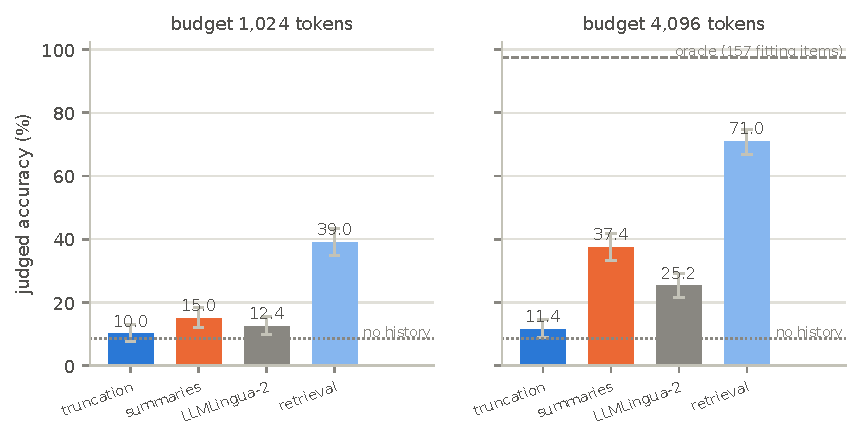
\includegraphics[width=\linewidth]{figures/fig_arms.pdf}\fi
\caption{Judged accuracy by policy at each budget, with Wilson 95\% intervals (500 questions per bar). The dotted line is the no-history control; the dashed oracle line covers only the fitting subset.}\label{fig:p5-arms}\end{figure}
\subsection{Does the order hold at 1,024 tokens, and do the variants change it?}\label{sec:budget}
At 1,024 tokens the four policies scored 39.0\% (retrieval), 15.0\% (summaries), 12.4\% (compression) and 10.0\% (truncation), the same order of point estimates as at 4,096 tokens, at lower levels. Against truncation at that budget, retrieval differed by +29.0 points [+24.7, +33.3], summaries by +5.0 [+2.4, +7.7] and compression by +2.4 [$-$0.4, +5.3] (Table~\ref{tab:p5-secondary}); compression (+2.4 points [$-$0.4, +5.3]) was not separated from truncation at that budget, and the alternatives were not tested against each other. At 4,096 tokens, BM25 ranking of past exchanges was not separated from MiniLM ranking (+2.2 points [$-$1.7, +6.1]), and compressing only the recent window instead of the whole history changed compression accuracy by $-$5.2 points [$-$9.7, $-$0.7]. Equal budgets did not give equal prompt lengths: at 1,024 tokens retrieval delivered 756 prompt tokens on average and compression 1,022, because retrieval stops at the first ranked round that does not fit (Figure~\ref{fig:p5-cost}). These comparisons are descriptive, and a contrast that is significant at one budget but not at the other does not by itself establish an interaction between policy and budget.

\begin{table}[htbp]\centering\small\setlength{\tabcolsep}{4pt}
\begin{tabular}{lrrr}\toprule
Comparison & Points & 95\% interval & Raw $p$\\ \midrule
S vs T, B=1024 & +5.0 & [+2.4, +7.7] & \ensuremath{2.47\times10^{-04}}\\
C vs T, B=1024 & +2.4 & [$-$0.4, +5.3] & 0.126347\\
M vs T, B=1024 & +29.0 & [+24.7, +33.3] & \ensuremath{6.77\times10^{-36}}\\
Cw vs T, B=1024 & +0.6 & [$-$1.3, +2.5] & 0.663624\\
Cw vs T, B=4096 & +8.6 & [+5.6, +11.7] & \ensuremath{3.38\times10^{-08}}\\
Mbm25 vs T, B=4096 & +61.8 & [+56.8, +66.2] & \ensuremath{2.53\times10^{-78}}\\
Cw vs C, B=4096 & $-$5.2 & [$-$9.7, $-$0.7] & 0.030415\\
Mbm25 vs M, B=4096 & +2.2 & [$-$1.7, +6.1] & 0.31488\\
\bottomrule\end{tabular}
\caption{Secondary paired contrasts, 500 items each, with pointwise Newcombe intervals and unadjusted McNemar p-values; descriptive, outside the three-test confirmatory family.}\label{tab:p5-secondary}
\end{table}
\subsection{Do the policies lose answers in selecting the text or in reading it?}\label{sec:selection}
Each policy has a diagnostic of how much annotated evidence its prompts kept, with its own denominator (Section~\ref{sec:statistics}); Figure~\ref{fig:p5-evidence} plots accuracy against it. At 4,096 tokens the prompts built by truncation held 3.8\% of the evidence turns and those built by retrieval 74.8\% (BM25 ranking: 79.0\%); summaries covered 44.0\% of the evidence sessions, and compression kept 26.3\% of the evidence words.
\begin{figure}[htbp]\centering
\ifdarkmode\includegraphics[width=\linewidth]{figures/dark/fig_evidence.pdf}\else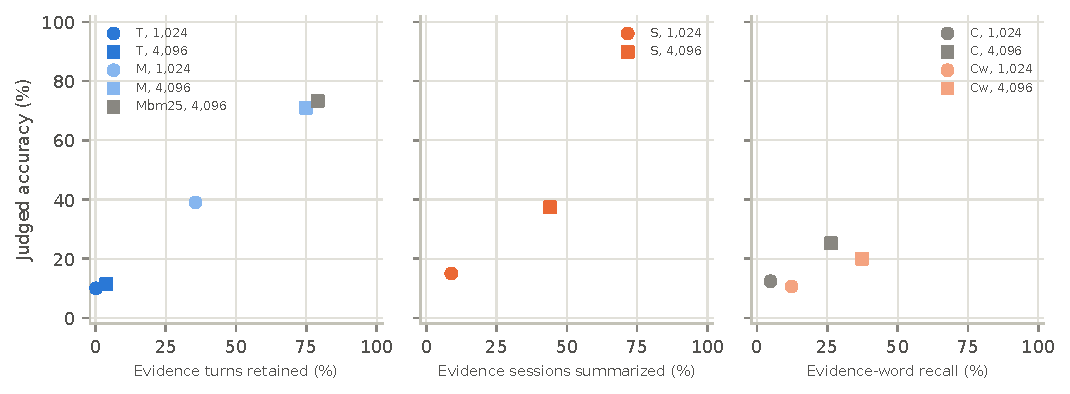
\includegraphics[width=\linewidth]{figures/fig_evidence.pdf}\fi
\caption{Accuracy against each policy's evidence diagnostic at both budgets (circles 1,024 tokens, squares 4,096). Retained evidence turns, summarized evidence sessions and evidence-word recall have different denominators and are plotted on separate axes (Section~\ref{sec:statistics}).}\label{fig:p5-evidence}\end{figure}

The oracle arm replaces selection with the annotated evidence: on the 157 questions whose evidence sessions fit 4,096 tokens, the generator was judged correct on 97.5\% when shown only those sessions (Table~\ref{tab:p5-oracle}). On the same questions retrieval trailed the oracle by 10.8 points, summaries by 51.0, compression by 69.4 and truncation by 84.1. On this subset the generator answered nearly every question when the evidence was all it saw, which points to selection as the main source of lost answers. The oracle prompt also omits all other history, so this comparison does not separate missing evidence from added distraction.

\begin{table}[htbp]\centering\small\setlength{\tabcolsep}{4pt}
\begin{tabular}{lrr}\toprule
Same-subset comparison & Points & 95\% interval\\ \midrule
O minus T & +84.1 & [+77.0, +88.7]\\
O minus S & +51.0 & [+42.2, +58.8]\\
O minus C & +69.4 & [+61.4, +75.9]\\
O minus M & +10.8 & [+5.9, +16.8]\\
\bottomrule\end{tabular}
\caption{Paired gaps between the oracle and each policy on the same 157 fitting items, the only items the oracle covers.}\label{tab:p5-oracle}
\end{table}
\subsection{Does the order hold across question types?}\label{sec:types}
Table~\ref{tab:p5-subgroups} splits accuracy by LongMemEval's declared question types. At 4,096 tokens the highest point estimate went to retrieval in all six types, with leads over truncation from 39.1 points (multi-session) to 87.5 points (single-session assistant). The 30 abstention questions, whose answer is absent from the history, overlap the types and put truncation first: truncation was credited on 30 of them, summaries on 24, compression on 25 and retrieval on 24. These groups are small, and the breakdown is descriptive; it does not test policy-by-type interactions.

\begin{table}[htbp]\centering\small\setlength{\tabcolsep}{4pt}
\begin{tabular}{lrrrrrr}\toprule
Budget & Question group & $n$ & T \% & S \% & C \% & M \%\\ \midrule
1,024 & Knowledge update & 78 & 11.5 & 23.1 & 17.9 & 47.4\\
1,024 & Multi-session & 133 & 9.8 & 10.5 & 6.8 & 18.0\\
1,024 & Single-session assistant & 56 & 12.5 & 19.6 & 10.7 & 87.5\\
1,024 & Single-session preference & 30 & 6.7 & 13.3 & 20.0 & 26.7\\
1,024 & Single-session user & 70 & 11.4 & 17.1 & 10.0 & 67.1\\
1,024 & Temporal reasoning & 133 & 8.3 & 12.0 & 15.0 & 22.6\\
1,024 & Abstention (overlaps types) & 30 & 100.0 & 93.3 & 73.3 & 86.7\\
4,096 & Knowledge update & 78 & 15.4 & 57.7 & 28.2 & 84.6\\
4,096 & Multi-session & 133 & 9.8 & 18.0 & 15.0 & 48.9\\
4,096 & Single-session assistant & 56 & 12.5 & 44.6 & 25.0 & 100.0\\
4,096 & Single-session preference & 30 & 6.7 & 40.0 & 26.7 & 63.3\\
4,096 & Single-session user & 70 & 17.1 & 44.3 & 31.4 & 90.0\\
4,096 & Temporal reasoning & 133 & 8.3 & 37.6 & 30.1 & 64.7\\
4,096 & Abstention (overlaps types) & 30 & 100.0 & 80.0 & 83.3 & 80.0\\
\bottomrule\end{tabular}
\caption{Primary-judge accuracy within each declared question group. Abstention overlaps the type rows; it is not an additional sample.}\label{tab:p5-subgroups}
\end{table}
\subsection{Does the order hold for another model and another benchmark?}\label{sec:transfer}
Two descriptive checks repeat the comparison outside the primary setting, each at 4,096 tokens. The first gives the same 500 questions and session summaries to Qwen3-8B, a smaller attention-only model from the same developer, served by llama.cpp with its own tokenizer and chat template (Table~\ref{tab:p5-crossmodel}). Retrieval again had the highest point estimate (64.2\%), and the four point estimates kept the order of the primary 27B run (M, S, C, T). This check changes the model and the serving stack together, so it isolates neither.

The second check uses 200 LoCoMo questions. A pre-specified rule chose M from S, M and C as the alternative with the most correct answers on the primary LongMemEval results; ties use that order, and selection does not require beating T. Because the rule selected retrieval, this check does not repeat the truncation-versus-summarization comparison that Kyrkewood ran on LoCoMo \citep{kyrkewood2026sleeping}. Retrieval was judged correct on 68.0\% of the questions against 17.0\% for truncation, a difference of +51.0 points (pointwise Newcombe interval [+42.3, +58.4], unadjusted McNemar $p=\ensuremath{1.71\times10^{-23}}$); these question-level calculations ignore that questions share conversation histories. Token F1 compares the whole visible answer with a short gold string, so every extra word lowers it and its level is low for both arms; it changed by +4.5 points, with a conversation-resampled 95\% interval of [+3.5, +5.7] over only 10 conversations (Table~\ref{tab:p5-locomo}). Neither result establishes general superiority across datasets.

\begin{table}[htbp]\centering\small\setlength{\tabcolsep}{4pt}
\begin{tabular}{lrrrrr}\toprule
Arm & Accuracy \% & 95\% interval & $\Delta$ vs T & 95\% interval & Raw $p$\\ \midrule
T & 10.8 & [8.4, 13.8] & -- & -- & --\\
S & 35.0 & [30.9, 39.3] & +24.2 & [+20.0, +28.4] & \ensuremath{1.69\times10^{-27}}\\
C & 17.8 & [14.7, 21.4] & +7.0 & [+3.5, +10.6] & \ensuremath{1.55\times10^{-04}}\\
M & 64.2 & [59.9, 68.3] & +53.4 & [+48.5, +57.9] & \ensuremath{7.44\times10^{-69}}\\
\bottomrule\end{tabular}
\caption{Qwen3-8B, 500 items per arm. Wilson accuracy and paired Newcombe difference intervals are pointwise; McNemar p-values are unadjusted and outside the primary Holm family.}\label{tab:p5-crossmodel}
\end{table}

\begin{table}[htbp]\centering\small\setlength{\tabcolsep}{4pt}
\begin{tabular}{lrrrr}\toprule
Arm & $n$ & Judged \% & Token-F1 \% & Cluster 95\% interval\\ \midrule
T & 200 & 17.0 & 3.9 & [3.3, 4.5]\\
M & 200 & 68.0 & 8.4 & [7.6, 9.5]\\
\bottomrule\end{tabular}
\caption{LoCoMo aggregates only. F1 percentile intervals resample whole conversations, with 10,000 draws and seed 20260920; the item-weighted mean is recomputed in every resample.}\label{tab:p5-locomo}
\end{table}
\subsection{Do the scores depend on the scorer?}\label{sec:scorers}
Scorer agreement is not validation against human correctness, and identical failure labels can inflate it, so the agreement rates below use only successful generations with a nonempty verdict from each compared scorer. No generation or verdict failed in any 4,096-token cell of the three runs, so the rule that scores failures as incorrect changed no accuracy. In the 27B run the local judge agreed with the generator acting as a second judge on 96.6--98.2\% of verdicts per policy ($\kappa$ 0.90--0.95), and with lexical containment of the gold answer on 78.0--91.4\% of short-answer items (Table~\ref{tab:p5-scorers}). In the 8B run the second judge, Qwen3-8B judging its own answers, agreed with the local judge on 69.4--87.2\% of verdicts ($\kappa$ 0.28--0.70); it enters no reported accuracy. In the 27B run the two judges' largest disagreement, 3.4\% of one policy's verdicts, is less than half the smallest gap between adjacent policies at 4,096 tokens (12.2 points), so scoring with the second judge could not have changed the order of the four policies; scored by lexical containment on the 440 short-answer items, the order was also unchanged (retrieval 55.7\%, summaries 34.5\%, compression 22.0\% and truncation 10.2\%). No agreement rate shows which scorer is correct. Every nonempty verdict in the displayed cells was a bare yes or no (allowing a final period), and no empty visible answer was credited; the upstream rule that credits any reply containing ``yes'' was kept unchanged.

\begin{table}[htbp]\centering\small\setlength{\tabcolsep}{4pt}
\begin{tabular}{llrrrrrr}\toprule
Run & Arm & Local--self \% & $\kappa$ & Local--lexical \% & $\kappa$ & Self--lexical \% & $\kappa$\\ \midrule
27B & T & 98.2 & 0.90 & 91.4 & 0.41 & 92.3 & 0.45\\
27B & S & 96.6 & 0.93 & 81.6 & 0.59 & 82.0 & 0.60\\
27B & C & 98.0 & 0.95 & 86.8 & 0.61 & 87.0 & 0.61\\
27B & M & 97.6 & 0.94 & 78.0 & 0.54 & 77.5 & 0.53\\
8B & T & 69.4 & 0.28 & 91.4 & 0.38 & 68.9 & 0.20\\
8B & S & 75.4 & 0.53 & 85.0 & 0.66 & 66.6 & 0.36\\
8B & C & 70.0 & 0.38 & 87.7 & 0.53 & 66.1 & 0.27\\
8B & M & 87.2 & 0.70 & 80.7 & 0.61 & 73.4 & 0.45\\
\bottomrule\end{tabular}
\caption{Scorer agreement on valid verdicts for the two LongMemEval deployments: the local judge (gpt-oss-20b), the generator as second judge (self) and lexical containment of the gold answer. Every scorer pair has its own denominator; these rates exclude failed verdicts and therefore differ from failure-coded agreement. Lexical comparisons exclude preference and abstention questions. Pair denominators per policy: local--self 500, local--lexical 440 and self--lexical 440.}\label{tab:p5-scorers}
\end{table}
\subsection{What did the policies cost in recorded time?}\label{sec:cost}
Figure~\ref{fig:p5-cost} shows the prompt tokens each policy delivered and the seconds recorded per question. At 4,096 tokens the four policies delivered 3,559--3,993 prompt tokens on average. Mean generation time per answer was 15.0\,s for truncation, 17.8\,s for retrieval, 19.2\,s for summaries and 24.9\,s for compression. Recorded selection added 0.19\,s for truncation, 0.42\,s for compression and 4.37\,s for retrieval, whose timer includes computing embeddings not already cached; summaries had no per-question selection timer. These timings follow policy-specific accounting boundaries and exclude summary generation, classifier preprocessing and the pause between requests (Section~\ref{sec:statistics}), so they do not rank the policies by end-to-end cost.
\begin{figure}[htbp]\centering
\ifdarkmode\includegraphics[width=\linewidth]{figures/dark/fig_cost.pdf}\else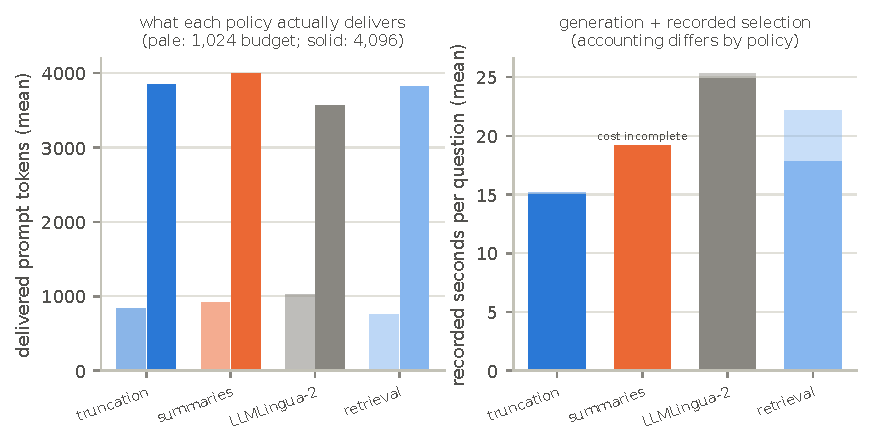
\includegraphics[width=\linewidth]{figures/fig_cost.pdf}\fi
\caption{Delivered prompt tokens (left) and recorded seconds per question at 4,096 tokens (right): generation plus the policy's recorded selection time, with accounting boundaries that differ by policy. Summary generation, classifier preprocessing and the pause between requests are excluded; retrieval's selection time includes embedding cache misses.}\label{fig:p5-cost}\end{figure}
\section{Discussion}\label{sec:discussion}
\paragraph{Measured pattern.} The policies filled similar token allowances with different material. At 4,096 tokens the prompts built by truncation held 3.8\% of the annotated evidence turns and those built by retrieval 74.8\%, and the two policies scored 11.4\% and 71.0\%. On the 157 questions whose evidence sessions fit, the generator was judged correct on 97.5\% when shown only those sessions (Section~\ref{sec:selection}). We infer that, for this generator, the policies differed mainly in how much evidence they put in front of the model: where two policies share a retention measure, retention and accuracy rise together, and on the fitting questions the model read the evidence almost perfectly. The oracle prompt also leaves out the rest of the history, so this inference does not exclude a contribution from distraction.

\paragraph{Possible mechanisms.} The design does not isolate why each policy lost evidence; the following explanations are consistent with the diagnostics but untested. LongMemEval-S spreads answer-bearing sessions throughout each history, so a recency window seldom reaches them: at 4,096 tokens truncation kept 17.7 of 493.5 messages on average. Session summaries reach further back (17.1 of 47.7 sessions) but were written before the question was known and are short, so a covered session can still lose the needed fact; their coverage of evidence sessions (44.0\%) bounds what they can supply from above. Whole-history compression runs far outside the range in which LLMLingua-2 was validated (Section~\ref{sec:policies}) and kept 26.3\% of the evidence words. Compressing only the recent window, inside that range, changed accuracy by $-$5.2 points [$-$9.7, $-$0.7] even though it kept more of the evidence words (37.3\%); word recall counts lexical overlap anywhere in the window, which may still omit the answer-bearing sessions. On abstention questions, more history may give the model material to answer from when it should decline, which would explain why truncation was credited on 30 of 30 and the other policies on 24--25.

\paragraph{Implications.} For an operator whose local assistant must answer questions about earlier sessions within a short prompt, the comparison favors retrieval over the whole history: it scored highest at both budgets and with Qwen3-8B, and it led truncation on LoCoMo. BM25 ranking, which needs no embedding model, was not separated from MiniLM ranking (+2.2 points [$-$1.7, +6.1]). On LongMemEval-S, whose evidence is spread through the history, recency truncation at the same budget scored 2.8 points above the no-history control at 4,096 tokens, so beating truncation alone says little about a new memory method on such benchmarks. Question-aware summaries or lighter compression might narrow the gap; this study did not test them.
}
\newcommand{\PfiveConclusion}{For Qwen3.8-27B, quantized to 2 bits per weight on a 12\,GB laptop GPU, answering LongMemEval-S questions about chat histories of more than 100,000 tokens within the same prompt budget for every policy, retrieval over the whole history preserved far more answers than session summaries, LLMLingua-2 compression or recency truncation: it was judged correct on 71.0\% of the questions at 4,096 tokens and 39.0\% at 1,024, against 11.4\% and 10.0\% for truncation. Its lead over truncation was confirmed by the pre-registered test; its lead over summaries and compression is descriptive. A local assistant that must answer questions about earlier sessions within a short prompt should start from retrieval over the full history rather than recency truncation, and evaluations on benchmarks like LongMemEval-S should not use truncation as their only baseline. These results are limited to the tested implementations, one primary generator, LongMemEval-S with a retrieval-versus-truncation check on LoCoMo, and local judges; they are not a ranking of memory policies in general or a measure of end-to-end cost.}
\newcommand{\PfiveFollowupSummary}{With Qwen3-8B, retrieval had the highest point estimate (64.2\%). On LoCoMo, retrieval, the alternative selected from the primary results, was judged correct on 68.0\% of 200 questions from 10 conversations against 17.0\% for truncation; its token-F1 difference from truncation was +4.5 points (conversation-resampled 95\% interval [+3.5, +5.7]). Both checks are descriptive.}
\newcommand{\PfiveFailureNote}{Four answers ended inside an unterminated thinking block (T 2, Cw 1 and O 1, all at 4,096 tokens) and were judged on their empty visible answers; one completion (C at 4,096 tokens) reached the completion cap.}
\newcommand{\PfiveLocomoConversations}{10}
\newcommand{\PfiveCap}{8,192}
